\icode{E-MI-SI-L3-261110-001}
如图所示，质量为\(M\)的光滑半圆柱体紧靠墙根放置，质量为\(m\)的小球由长度为\(L\)的细线悬挂于竖直墙壁上的\(A\)点，静止在半圆柱体上，\(A\)点距离地面的高度为\(L\)，细线与竖直方向夹角为\(\theta\)。已知半圆柱体的半径可变化(质量不变)，小球可视为质点，重力加速度为\(g\)，不计一切摩擦，下列说法正确的是\paren[]

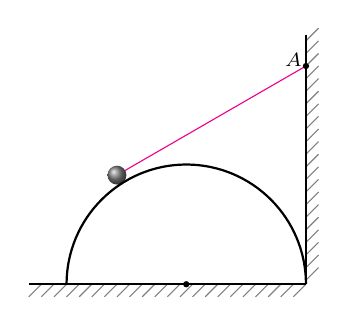
\begin{tikzpicture}[scale=.8,font=\scriptsize]
	\draw[magenta] (0,0)--(-150:{2*sqrt(3)});
	\shade[ball color=gray] (-150:{2*sqrt(3)}) circle(.15);
	\draw[thick] (0,{-2*sqrt(3)}) arc(0:180:1.9); 
	\foreach \x in {-4.4,-4.2,...,-.2}
		\draw[gray] (\x,{-2*sqrt(3)-0.2})--++(.2,.2);
	\foreach \y in {-3.4,-3.2,...,.4}
		\draw[gray] (0,\y)--++(.2,.2);
	\draw[thick] (-4.4,{-2*sqrt(3)})--(0,{-2*sqrt(3)}) (0,.5)--(0,{-2*sqrt(3)});
	\node at(-.2,.1){\(A\)};
	\fill (-1.9,{-2*sqrt(3)}) circle(.05) (0,0) circle(.05);
\end{tikzpicture}
\begin{choices}
	\item 当\(\theta =\)\,\qty{60}{\degree}时，细线对小球的拉力大小为\(\frac{\sqrt{3}}{2}mg\)
	\item 当\(\theta =\)\,\qty{60}{\degree}时，半圆柱体对小球的支持力大小为\(\frac{1}{2}mg\)
	\item 半圆柱体受到水平地面的弹力大小为\(Mg + mg\sin^2\theta\)
	\item 半圆柱体受到竖直墙壁的弹力最大值为\(mg\)
\end{choices} 
\begin{answer}
	C\qquad 提示：
\end{answer}